% !TEX root = ../chap2.tex

\section{Comparaison des deux résolutions hybrides}
\label{s:compare}

Dans cette section on s'intéressera à la comparaison des méthodes de simulation présentées dans la section~\ref{s:scheme} pour 
approcher num\'eriquement le mod\`ele VHL. On \'etudiera en particulier les méthodes de pas de temps adaptatif associées. 
Nous utilisons dans cette section la condition initiale suivante :
$$
  \begin{aligned}
    u_c(x)   &= 0 \\
    f_h(x,v) &=  \left(\mathcal{M}_{^\alpha/_2,v_0,1}(v) +  \mathcal{M}_{^\alpha/_2,-v_0,1}(v) \right)(1 + \epsilon\cos(kx))
  \end{aligned}
$$
avec $k=0.5$, $\alpha=0.2$, $v_0 = 4$, $x\in [0,4\pi]$, $v\in[-8,8]$, et la perturbation $\epsilon = 0.1$. Le champ électrique initiale $E(t=0,x)$ est obtenu en résolvant l'équation de Poisson sur notre condition initiale, comme indiqué dans la proposition~\ref{p:vhl_conservation} :
$$
  \partial_x E(t=0) = (1-\alpha) + \int (1+\epsilon\cos(kx))\left( \mathcal{M}_{^\alpha/_2,v_0,1}(v) + \mathcal{M}_{^\alpha/_2,-v_0,1}(v) \right)\,\mathrm{d}v - 1
$$
La discrétisation du domaine s'effectue avec $N_x=81$ dans la direction $x$, et $N_v=128$ points dans la direction $v$.

Nous allons effectuer différentes configurations pour tester et comparer les deux m\'ethodes 
\begin{enumerate}
\item pas de temps fixe 
\begin{itemize}
\item  $\Delta t = 0.5\Delta v$ 
\item  $\Delta t = \sigma\frac{\Delta t}{\|E^n\|_\infty}$ où $\sigma \approx 1.433$ est la condition CFL de WENO5 avec DP4, et $\|E^n\|_\infty = \max_{t^n}(\max_i|E_i^n|) \approx 0.2$ d'après une estimation issue des résultats d'une simulation ; 
\item  $\Delta t = 1$ qui est un pas de temps choisi arbitrairement grand pour illustrer l'absence de condition CFL de la méthode de Suzuki. 
\end{itemize}
\item pas de temps adaptatif
\begin{itemize}
\item méthode présentée dans la section~\ref{ssec:dtadapt} avec une tolérance $tol = 10^{-4}$, 
\item méthode basée sur la condition de CFL en choisissant $\Delta t^n = \min\left(\sigma\frac{\Delta v}{\|E^n_i\|_\infty},2\right)$ où $\sigma \approx 1.433$, et $\|E_i^n\|_\infty = \max_i\left( |E^n_i|\right)$.
\end{itemize}
\end{enumerate}
Quelque soit la méthode de simulation choisie, nous allons regarder les estimateurs d'erreur présentées dans la section~\ref{ssec:dtadapt} :
$$
  \begin{aligned}
    L &= \left(\sum_i (\left.u_c\right.^{[4]}_i-\left.u_c\right.^{[3]}_i)^2\Delta x\right)^{\frac{1}{2}}
          + \left(\sum_i (\left.E\right.^{[4]}_i-\left.E\right.^{[3]}_i)^2\Delta x\right)^{\frac{1}{2}}
          + \left(\sum_{i,j} \left|\left.{f}_h\right.^{[4]}_{i,j}-\left.{f}_h\right.^{[3]}_{i,j}\right|^2\Delta v\Delta x\right)^{\frac{1}{2}} \\
      &= L_{u_c} + L_{E} + L_{{f}_h}
  \end{aligned}
$$
Cela permettra de comparer l'estimation de l'erreur avec une même tolérance entre la méthode DP4(3) et la méthode de Suzuki. Nous allons aussi regarder le nombre d'itération de chaque méthode de simulation, et la taille des pas de temps que la méthode de pas de temps adaptatif propose. Il est à noter que uniquement les deux méthodes de la section~\ref{ssec:dtadapt} utilisent cette estimation d'erreur et ont un critère pour rejeter une itération.

\commentaire[Nicolas]{Figure 9 : en faire 2 figure (Suzuki et DP par exemple ?). Reprendre les commentaires en fonction du coup. }
\begin{figure}[h]
  \centering
  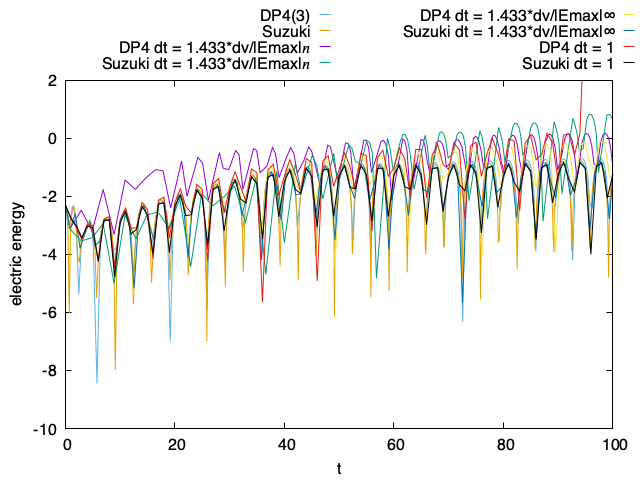
\includegraphics[width=0.8\textwidth]{img/compare_ee.png}
  \caption{Évolution de l'énergie électrique avec les différentes méthodes}
  \label{fig:compare:ee}
\end{figure}

Sur la figure~\ref{fig:compare:ee} on peut voir l'évolution de l'énergie électrique au cours du temps pour les différentes simulations. Il est important de remarquer que 4 résultats sont différents de ce que prédit la relation de dispersion, la courbe rouge, qui est un résultat donné par la méthode DP4 avec un pas de temps $\Delta t=1$ hors de la condtion CFL, le schéma est instable ; la courbe jaune, dont les résultats sont donnés par la méthode DP4 avec un pas de temps $\Delta t=1.433\Delta v/\|E\|_\infty$ est l'illustration d'un schéma utilisé juste sous sa condition de CFL, le schéma est stable mais il n'est pas précis ; les courbes violettes et vertes sont issus des résultats respectivement de DP4 et Suzuki avec une méthode de pas de temps adaptatif donné par la condition de CFL, cette méthode de pas de temps adaptatif propose de très grand pas de temps dans la phase linéaire du problème où le champ électrique est faible, mais produit une erreur importante, qui se répercute sur les résultats en fin de simulation. Les autres résultats sont conformes aux relations de dispersion. 

\begin{figure}[h]
  \centering
  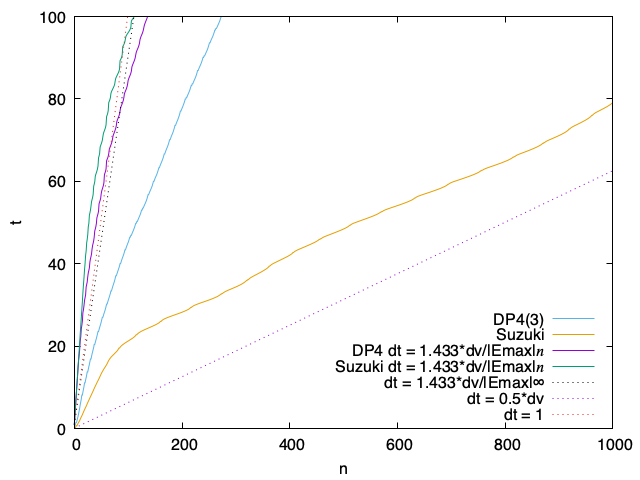
\includegraphics[width=0.8\textwidth]{img/compare_time_dtt}
  \caption{Évolution du temps au cours des itérations de la simulation}
  \label{fig:compare:time:dtt}
\end{figure}

Sur la figure~\ref{fig:compare:time:dtt} on représente l'évolution du temps courant dans la simulation en fonction des itérations. Les courbes en pointillés sont celles avec un pas de temps constant. On remarque que les simulations où le pas de temps est guidé par la condition de CFL locale sont parmi les plus performantes pour atteindre le temps final, mais comme nous avons pu le voir sur la figure précédente~\ref{fig:compare:ee}, ce sont aussi celles qui donnent des résultats avec une très mauvaise précision. Les simulations avec un pas de temps constant très grand, donnent à première vue de bon résultat avec un intégrateur en temps sans condition de CFL comme Suzuki, mais de mauvais résultats avec la méthode DP4. La méthode DP4(3) s'impose ensuite comme un très bon choix pour maintenir l'erreur sous une certaine tolérance tout en atteignant rapidement le temps final, ici $T_f=100$. Les résultats pour la méthodes de Suzuki à pas de temps adaptatif ou les simulations avec un pas de temps pris arbitrairement petit $\Delta t = 0.5\Delta v$, ont été tronqués pour mieux observer les simulations plus rapide, la méthode de Suzuki termine en 1290 itérations, et les simulations avec un pas de temps fixé à $\Delta t = 0.5\Delta v$ en 1600 itérations.
commentaire[Nicolas]{Je ne comprends pas bien la fin : pourquoi 2 m\'ethodes ont \'et\'e "tronqu\'ees" ? }

\begin{figure}[h]
  \centering
  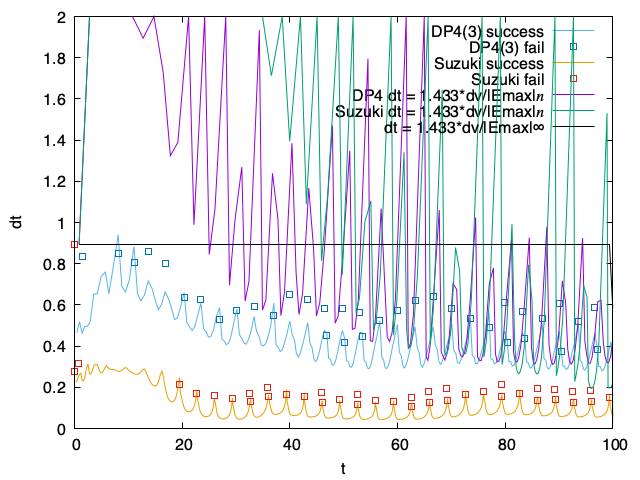
\includegraphics[width=0.8\textwidth]{img/compare_dt_cfl.png}
  \caption{Évolution de la taille du pas de temps $\Delta t^n$ au cours du temps, les itérations rejetées sont notées à l'aide des carrés}
  \label{fig:compare:dt:all}
\end{figure}

Il est intéressant de regarder, pour des méthodes à pas de temps adaptatif, l'évolution de la taille du pas de temps. C'est ce qui est tracé sur la figure~\ref{fig:compare:dt:all} en fonction du temps, les itérations rejetées par un critère d'erreur n'ont pas été représentées sur cette figure. Les simulations dont le pas de temps est donné par la condition de CFL locale $\sigma \Delta v/(\max |E^n|)$ (en violet et en vert sur la figure) sont soumis à de très importantes variations dans le choix du pas de temps, de plus, pour éviter des erreurs trop importantes en début de simulation, il a été choisi de toujours prendre un pas de temps inférieur à 2, cette forte variabilité dans le choix du pas de temps implique une erreur relativement importante dans les résultats. La méthode DP4(3) propose des pas de temps autour de $0.5$ et propose des pas de temps plus important dans la phase linéaire (entre les temps 5 et 40). La méthode de Suzuki, alors qu'elle n'est soumis à aucune condition de stabilité, propose des pas de temps bien plus faible, jusqu'à proposer des pas de temps similaire au choix arbitraire $\Delta t = 0.5\Delta v$, et ce avant l'installation de la saturation de l'énergie électrique au temps 40. Sur la figure~\ref{fig:compare:dt} on représente à la fois les itérations acceptées et rejetées par le critère d'erreur, on remarque que le pas de temps des itérations rejetées reste du même ordre de grandeur que les autres itérations. Les rejets d'itérations ont toujours lieu lors des rebonds de l'énergie électrique, pour éviter trop de rejets de la sorte, il est possible de limiter les évolutions du pas de temps de l'itération suivante avec par exemple $\Delta t^{n+1} \in [0.5\Delta t^n,2\Delta t^n]$. \commentaire[Nicolas]{Dire que si on rejete moins, on va plus vite...)}
\commentaire[Nicolas]{Il faudrait parler des courbes "fail" de la figure 11 ; j'imagine que ce sont les iterations rejetees ?}


\begin{figure}[h]
  \centering
  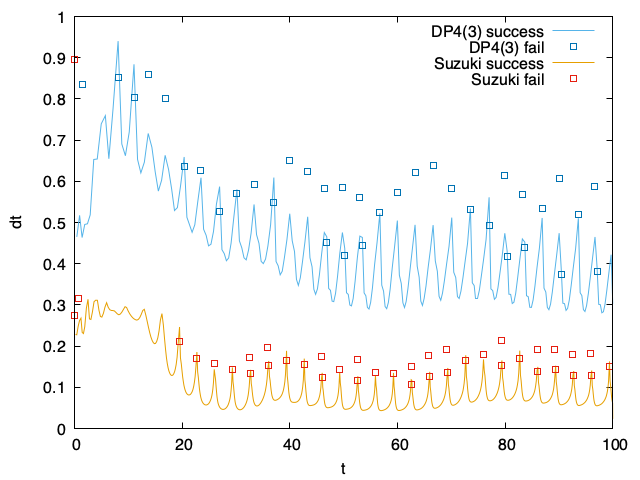
\includegraphics[width=0.8\textwidth]{img/compare_dt.png}
  \caption{Évolution de la taille du pas de temps $\Delta t^n$ au cours du temps, les itérations rejetées sont notées à l'aide des carrés}
  \label{fig:compare:dt}
\end{figure}

On peut regarder l'évolution de l'erreur estimée $L$ au cours du temps de la simulation sur la figure~\ref{fig:compare:error_dtt}, ici encore les itérations rejetées par le critère sont représentées différemment. Les deux méthodes effectuent dans les itérations acceptées une erreur similaire qui semble tourner autour de $0.5 tol$. On peut également combiner les résultats de la figure~\ref{fig:compare:dt} avec ceux de la figure~\ref{fig:compare:error_dtt} pour tracer le nuage de points de l'erreur commise à chaque itération en fonction du pas de temps proposé par la méthode, ce que l'on trace sur la figure~\ref{fig:compare:error:dt}. On remarque que de manière général la méthode DP4(3) propose des pas de temps plus grand, et pour chaque méthode, ce ne sont pas les itérations avec les plus grands pas de temps qui sont rejetées. La méthode de Suzuki semble ne jamais effectuer une erreur qui excède $2tol$.

\begin{figure}[h]
  \centering
  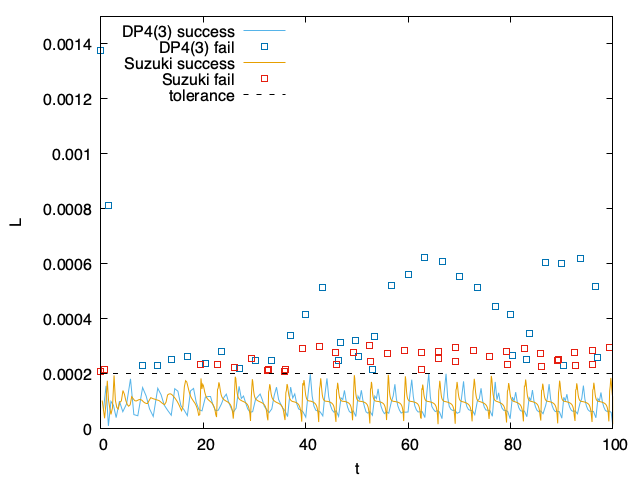
\includegraphics[width=0.8\textwidth]{img/compare_error_dtt.png}
  \caption{Étude de l'erreur $L$ au cours du temps, l'erreur des itérations rejetées est notée à l'aide des carrés}
  \label{fig:compare:error_dtt}
\end{figure}

\begin{figure}[h]
  \centering
  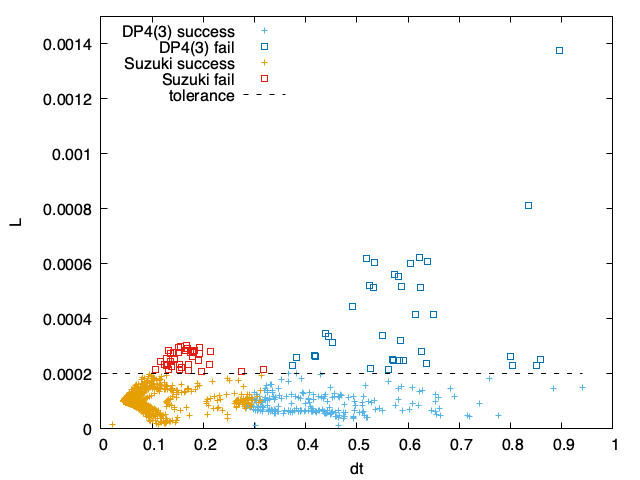
\includegraphics[width=0.8\textwidth]{img/compare_error_dt.png}
  \caption{Comparaison de l'erreur commise en fonction de la taille du pas de temps}
  \label{fig:compare:error:dt}
\end{figure}

Regardons, toujours pour ces 2 méthodes, l'évolution de l'erreur au cours du temps, mais en regardant la contribution dans $L$ d\^ue à $L_{u_c}$, $L_E$ et $L_{\hat{f}_h}$. C'est ce que l'on représente dans la figure~\ref{fig:compare:error:LucEfh}. L'erreur de la méthode DP4(3) et ses différentes contributions est représentée en haut, alors que celle de la méthode de Suzuki est représentée en bas. La méthode de Lawson propose de résoudre exactement la partie linéaire du problème, dans notre cas seul $u_c$ est entièrement résolu par la partie linéaire, ce qui explique une contribution à l'erreur de l'ordre de $10^{-18}$ pour $L_{u_c}$. La partie non linéaire comprend le calcul du courant de $f_h$ dans $L_E$, et le transport dans la direction $v$ dans $L_{\hat{f}_h}$, ces 2 composantes restent élevées tout au long de la simulation. Pour la méthode de Suzuki, l'erreur provient essentiellement de $L_{\hat{f}_h}$, ce qui est  li\'e \`a l'erreur 
produite par la méthode Lagrange 5 pour la résolution du transport dans la direction $v$.

\begin{figure}[h]
  \centering
  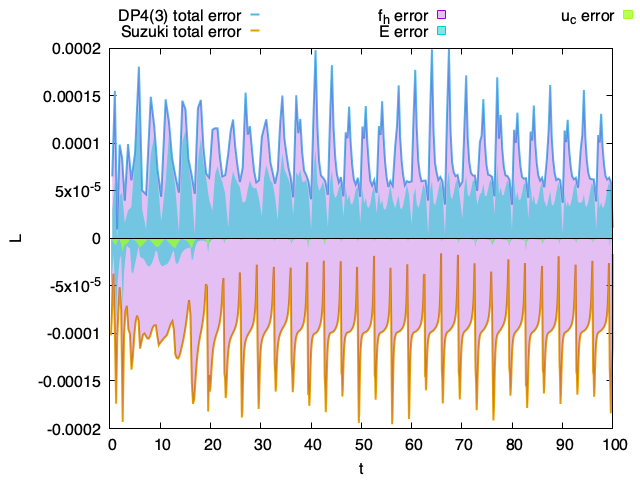
\includegraphics[width=0.8\textwidth]{img/compare_error_LucEfh.png}
  \caption{Comparaison de l'erreur au cours du temps et de la contribution de chaque composante de l'erreur}
  \label{fig:compare:error:LucEfh}
\end{figure}

%\commentaire[Nicolas]{Il faut expliquer comment tu calcules l'erreur pour les methodes non-embedded. J'imagine que tu calcules l'erreur locale 
%comme avec le pas de temps adaptatif mais sans changer le pas de temps avec la formule ? 
%On peut aussi regarder l'évolution de l'erreur sur toutes les simulations effectuées, quelque soit la méthode d'intégration en temps et le choix du pas de temps. C'est ce qui est effectué sur la figure~\ref{fig:compare:error:dtc} où l'on trace l'évolution de l'erreur en échelle semi-log. 
\commentaire[Nicolas]{Quelque soit le choix du pas de temps, on peut utiliser les estimateurs d'erreur locale pour \'etudier l'\'evolution de l'erreur au cours du temps 
pour les diff\'erentes m\'ethodes. C'est l'objet de la figure~\ref{fig:compare:error:dtc} où l'on trace l'évolution de l'erreur en échelle semi-log 
pour diff\'erentes m\'ethodes ainsi que la tol\'erance $10^{-4}$.}
On remarque que l'erreur commise par la méthode de Suzuki et DP4(3) est bien plus faible que les autres méthodes, et ce d'environ deux ordres de grandeur. Il n'y a que les simulations avec un pas fixe $\Delta t = 0.5\Delta v$ qui sont également sous la tolérance  fixé \`a 
$10^{-4}$. Donc sans connaissance a priori du problème, les méthodes à pas de temps adaptatif présentées dans la section~\ref{ssec:dtadapt} sont très intéressantes. Nous pouvons aussi remarquer que la constante d'erreur en temps de la méthode de Suzuki est bien plus importante que la méthode DP4(3) en regardant pour des simulations avec un pas de temps fixe l'erreur commise (par exemple les courbes en pointillées), ceci explique pourquoi la méthode DP4(3) propose des pas de temps plus important pour la même tolérance.

\begin{figure}[h]
  \centering
  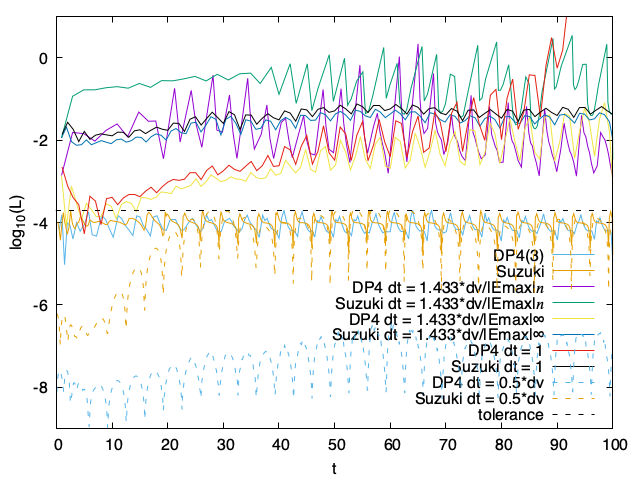
\includegraphics[width=0.8\textwidth]{img/compare_error_dtc.png}
  \caption{Comparaison de l'erreur obtenue à l'aide du temps de temps adaptatif et d'un pas de temps constant}
  \label{fig:compare:error:dtc}
\end{figure}



\commentaire[Nicolas]{Tracer l'energie totale pour differentes methods (pas de temps fixe Suzuki(dt=1 et dt=2) et DP4(3) + Suzuki en dt adaptatif) }
\commentaire[Nicolas]{temps de calcul par iteration et par etape de calcul. }

